\PassOptionsToPackage{unicode=true}{hyperref} % options for packages loaded elsewhere
\PassOptionsToPackage{hyphens}{url}
%
\documentclass[11pt,ignorenonframetext,]{beamer}
\usepackage{pgfpages}
\setbeamertemplate{caption}[numbered]
\setbeamertemplate{caption label separator}{: }
\setbeamercolor{caption name}{fg=normal text.fg}
\beamertemplatenavigationsymbolsempty
% Prevent slide breaks in the middle of a paragraph:
\widowpenalties 1 10000
\raggedbottom
\setbeamertemplate{part page}{
\centering
\begin{beamercolorbox}[sep=16pt,center]{part title}
  \usebeamerfont{part title}\insertpart\par
\end{beamercolorbox}
}
\setbeamertemplate{section page}{
\centering
\begin{beamercolorbox}[sep=12pt,center]{part title}
  \usebeamerfont{section title}\insertsection\par
\end{beamercolorbox}
}
\setbeamertemplate{subsection page}{
\centering
\begin{beamercolorbox}[sep=8pt,center]{part title}
  \usebeamerfont{subsection title}\insertsubsection\par
\end{beamercolorbox}
}
\AtBeginPart{
  \frame{\partpage}
}
\AtBeginSection{
  \ifbibliography
  \else
    \frame{\sectionpage}
  \fi
}
\AtBeginSubsection{
  \frame{\subsectionpage}
}
\usepackage{lmodern}
\usepackage{amssymb,amsmath}
\usepackage{ifxetex,ifluatex}
\usepackage{fixltx2e} % provides \textsubscript
\ifnum 0\ifxetex 1\fi\ifluatex 1\fi=0 % if pdftex
  \usepackage[T1]{fontenc}
  \usepackage[utf8]{inputenc}
  \usepackage{textcomp} % provides euro and other symbols
\else % if luatex or xelatex
  \usepackage{unicode-math}
  \defaultfontfeatures{Ligatures=TeX,Scale=MatchLowercase}
\fi
\usetheme[]{Szeged}
\usecolortheme{spruce}
% use upquote if available, for straight quotes in verbatim environments
\IfFileExists{upquote.sty}{\usepackage{upquote}}{}
% use microtype if available
\IfFileExists{microtype.sty}{%
\usepackage[]{microtype}
\UseMicrotypeSet[protrusion]{basicmath} % disable protrusion for tt fonts
}{}
\IfFileExists{parskip.sty}{%
\usepackage{parskip}
}{% else
\setlength{\parindent}{0pt}
\setlength{\parskip}{6pt plus 2pt minus 1pt}
}
\usepackage{hyperref}
\hypersetup{
            pdftitle={Prediction and analysis of the residential buildings permits},
            pdfborder={0 0 0},
            breaklinks=true}
\urlstyle{same}  % don't use monospace font for urls
\newif\ifbibliography
\setlength{\emergencystretch}{3em}  % prevent overfull lines
\providecommand{\tightlist}{%
  \setlength{\itemsep}{0pt}\setlength{\parskip}{0pt}}
\setcounter{secnumdepth}{0}

% set default figure placement to htbp
\makeatletter
\def\fps@figure{htbp}
\makeatother

\usepackage{setspace}

% to make the first rows bold in tables
\usepackage{longtable}
\usepackage{tabu}
\usepackage{booktabs}

% Floats
\usepackage{morefloats}
\usepackage{float}
\usepackage{placeins}

% highlighting
\usepackage{soul}

% Short toc
\usepackage{shorttoc}
\setcounter{tocdepth}{1}

% referencing mutliple things with a single command - \cref
% \usepackage{cleveref}

% longtables
\usepackage{longtable}

% Change section names style
% \usepackage[dvipsnames]{xcolor}
% \usepackage{sectsty}
\logo{\includegraphics[height = 10mm]{../images/logouga.png}
  \hspace{9.8cm} \includegraphics[height = 10mm]{../images/logoshnd.jpg}}

% \sectionfont{\color{Green}}  % sets colour of sections
% \subsectionfont{\color{Green}}  % sets colour of sub
% \subsubsectionfont{\color{Green}}  % sets colour of subsub

% this makes dots in table of contents
% \renewcommand{\cftsecleader}{\cftdotfill{\cftdotsep}}
% to change the title of contents
% \renewcommand{\contentsname}{Whatever}

% line numbers for review purposes
% this package might not be available in default latex installation 
% get it by 'sudo tlmgr install lineno'
%\usepackage{lineno}
%\linenumbers

% Array
\usepackage{array}
\usepackage{makecell}

% Multiple columns
\usepackage{multicol}

% Image insertion and colors
\usepackage{graphicx}

% to be able to include latex comments
\newenvironment{dummy}{}{}

\makeatletter
\setbeamertemplate{footline}{%
  \leavevmode%
  \hbox{%
  \begin{beamercolorbox}[wd=.333333\paperwidth,ht=2.25ex,dp=1ex,center]{author in head/foot}%
    \usebeamerfont{author in head/foot}{J.Mao, N.Gusarov, T.Viellescazes}
  \end{beamercolorbox}%
  \begin{beamercolorbox}[wd=.333333\paperwidth,ht=2.25ex,dp=1ex,center]{title in head/foot}%
    \usebeamerfont{institute in head/foot}\insertshortinstitute
  \end{beamercolorbox}%
  \begin{beamercolorbox}[wd=.333333\paperwidth,ht=2.25ex,dp=1ex,right]{date in head/foot}%
    \usebeamerfont{date in head/foot}\insertshortdate{}\hspace*{2em}
   %\insertframenumber{} / \inserttotalframenumber\hspace*{2ex} % old version
    \insertframenumber{} \hspace*{2ex} % new version without total frames
  \end{beamercolorbox}}%
  \vskip0pt%
}
\makeatother

\title{Prediction and analysis of the residential buildings permits}
\providecommand{\subtitle}[1]{}
\subtitle{Schnieder project}
\author{Justine Mao, Nikita Gusarov, Tom Vieillescazes\\
\tiny{Under direction of Beatrice Roussillon and Mathias Verdiere}}
\providecommand{\institute}[1]{}
\institute{Université Grenoble Alpes}
\date{10 january 2020}

\begin{document}
\frame{\titlepage}

\hypertarget{introduction}{%
\section{Introduction}\label{introduction}}

\begin{frame}{Objectives}
\protect\hypertarget{objectives}{}

\begin{itemize}
\tightlist
\item
  Analyse the factors influencing construction permits number.
\item
  Elaborate a predictive model for the construction permits to be
  issued.
\end{itemize}

\end{frame}

\begin{frame}{Presentation plan}
\protect\hypertarget{presentation-plan}{}

\begin{itemize}
\tightlist
\item
  Litterature study presentation
\item
  Database construction
\item
  Data presentation
\item
  Data analysis
\item
  Modelisation

  \begin{itemize}
  \tightlist
  \item
    Simple OLS models
  \item
    Time series models
  \item
    Alternative models
  \end{itemize}
\end{itemize}

\end{frame}

\hypertarget{litterature}{%
\section{Litterature}\label{litterature}}

\begin{frame}{Sources}
\protect\hypertarget{sources}{}

Nous avons commencé notre étude de la littérature par la recherche des
articles méthodologiques et théoriques en lien avec le sujet traité.

Les moteurs de recherche scientifique les plus utilisés ont été :

\begin{itemize}
\tightlist
\item
  Science Direct
\item
  Google Scholar
\item
  Elsevier
\item
  SAGE journals
\end{itemize}

\end{frame}

\begin{frame}{Variables of interest}
\protect\hypertarget{variables-of-interest}{}

\tiny
\begin{table}[H]
\begin{tabular}{p{6cm} | c}
\hline \\[-1.8ex]
Number of building permits postponed by one quarter (French Building Federation, 2017) & + \\
\hline
10-year OAT rate lagged by two quarters (French Building Federation, 2017) & - \\
\hline
Unemployment rate lagged by two quarters (French Building Federation, 2017) & - \\
\hline
Deadline for housing outstandings in quarter sales shifted by one quarter (French Building Federation, 2017) & - \\
\hline
Political measure (French Building Federation, 2017)
& + or - \\
\hline
Age of the population (Lindh et al, 2008) & \\
- Individus moins de 20 ans & ++ \\
- Individuals between 20 and 59 years old (National Institute for Demographic Studies, 2019) & + \\
- Individuals over the age of 75 & -  \\
\hline
Real estate prices (Essay et al, 2015) & - \\
\hline
GDP (Lindh et al, 2002) & + \\
\hline
\end{tabular}
\normalsize
\caption{Variables of interest}
\end{table}

\end{frame}

\hypertarget{database}{%
\section{Database}\label{database}}

\begin{frame}{Data sources}
\protect\hypertarget{data-sources}{}

We construct our database using macroeconomical variables figuring in
different french and international databases :

\begin{itemize}
\tightlist
\item
  Eurostat
\item
  \href{mailto:Sit@del2}{\nolinkurl{Sit@del2}}
\item
  INSEE
\item
  OCDE
\end{itemize}

\end{frame}

\begin{frame}{Data already studied}
\protect\hypertarget{data-already-studied}{}

The variables that we have already presented are :

\begin{itemize}
\tightlist
\item
  Number of the building permits,
\item
  Surface authorised for construction (not used in analysis anymore),
\item
  GDP,
\item
  Long term interest rate,
\item
  Households spendings,
\item
  Households investments.
\end{itemize}

\end{frame}

\begin{frame}{Changes and advances}
\protect\hypertarget{changes-and-advances}{}

We have extracted as well the following variables :

\begin{itemize}
\tightlist
\item
  Population part by age group :

  \begin{itemize}
  \tightlist
  \item
    less than 20 years old,
  \item
    from 20 to 59 years old,
  \item
    from 60 years and more.
  \end{itemize}
\item
  Proxy variables serving to capture policies changes :

  \begin{itemize}
  \tightlist
  \item
    elective cycles dummy variables,
  \item
    political party appartainance.
  \end{itemize}
\item
  Real estate housing prices,
\item
  Household confidence index.
\end{itemize}

\end{frame}

\hypertarget{data}{%
\section{Data}\label{data}}

\begin{frame}{Descriptive statistics}
\protect\hypertarget{descriptive-statistics}{}

\FloatBarrier

\tiny

\begin{table}[!htbp] \centering 
\begin{tabular}{@{\extracolsep{5pt}}lcccc} 
\\[-1.8ex]\hline 
\hline \\[-1.8ex] 
Statistic & \multicolumn{1}{c}{Mean} & \multicolumn{1}{c}{St. Dev.} & \multicolumn{1}{c}{Min} & \multicolumn{1}{c}{Max} \\ 
\hline \\[-1.8ex] 
Year & 2,006.000 & 7.360 & 1,994 & 2,018 \\ 
GDP & 1,956.328 & 219.289 & 1,545.800 & 2,285.900 \\ 
Interest rate & 3.903 & 1.867 & 0.468 & 7.535 \\ 
Household spendings & 1,018.228 & 122.541 & 801.300 & 1,186.200 \\ 
Household investments & 111.336 & 12.820 & 87.300 & 134.800 \\ 
Number of permits & 381,173.600 & 70,800.620 & 275,711 & 526,592 \\ 
Population < 20 y.o. & 25.007 & 0.686 & 24.003 & 26.370 \\ 
Population 20-59 y.o. & 52.887 & 1.389 & 49.991 & 54.176 \\ 
Population > 60 y.o. & 22.105 & 1.964 & 19.882 & 26.006 \\ 
\hline \\[-1.8ex] 
\end{tabular} 
  \caption{Descriptivve statistics for annual data} 
  \label{} 
\end{table}

\normalsize

\FloatBarrier

\end{frame}

\begin{frame}{Data transformation}
\protect\hypertarget{data-transformation}{}

In our work we prefer to operate over indiced variables.

\FloatBarrier

\tiny

\begin{table}[!htbp] \centering 
\begin{tabular}{@{\extracolsep{5pt}}lcc} 
\\[-1.8ex]\hline 
\hline \\[-1.8ex] 
Statistic & \multicolumn{1}{c}{Mean} & \multicolumn{1}{c}{St. Dev.} \\ 
\hline \\[-1.8ex] 
Year & 12.000 & 7.360 \\ 
GDP & 1.017 & 0.014 \\ 
Interest rate & 0.936 & 0.238 \\ 
Household spendings & 1.017 & 0.011 \\ 
Household investments & 1.014 & 0.041 \\ 
Number of permits & 1.022 & 0.148 \\ 
Population < 20 y.o. & 0.996 & 0.002 \\ 
Population 20-59 y.o. & 0.997 & 0.004 \\ 
Population > 60 y.o. & 1.011 & 0.007 \\ 
\hline \\[-1.8ex] 
\end{tabular} 
  \caption{Descriptive statistics for transformed data} 
  \label{} 
\end{table}

\normalsize

\FloatBarrier

\end{frame}

\begin{frame}{Graphical representation}
\protect\hypertarget{graphical-representation}{}

\FloatBarrier

\tiny

\begin{figure}[!htbp]

{\centering 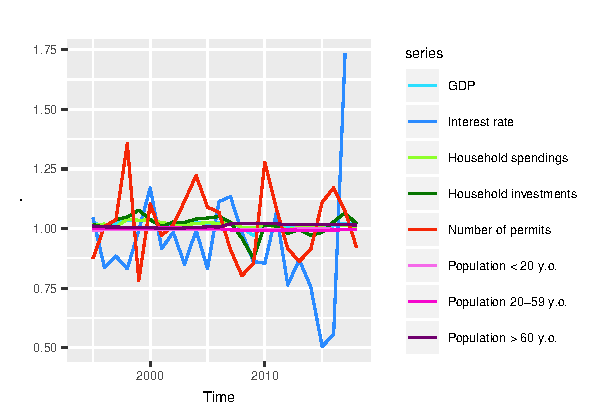
\includegraphics{presentation_files/figure-beamer/unnamed-chunk-12-1} 

}

\caption{Original data}\label{fig:unnamed-chunk-12}
\end{figure}

\normalsize

\FloatBarrier

\end{frame}

\begin{frame}{Political changes}
\protect\hypertarget{political-changes}{}

\FloatBarrier

\tiny

\begin{figure}[!htbp]

{\centering 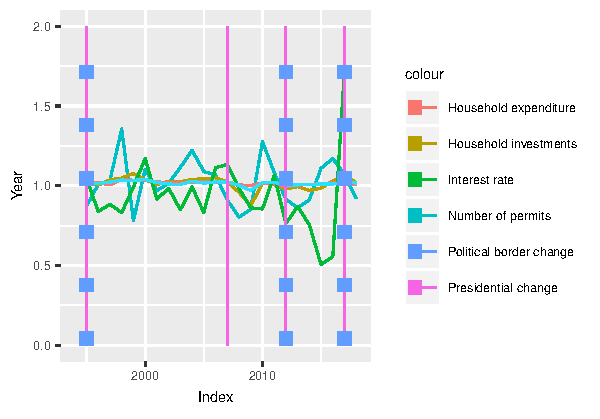
\includegraphics{presentation_files/figure-beamer/unnamed-chunk-14-1} 

}

\caption{Original data}\label{fig:unnamed-chunk-14}
\end{figure}

\normalsize

\FloatBarrier

\end{frame}

\begin{frame}{Different housing types}
\protect\hypertarget{different-housing-types}{}

\FloatBarrier

\tiny

\begin{figure}[!htbp]

{\centering 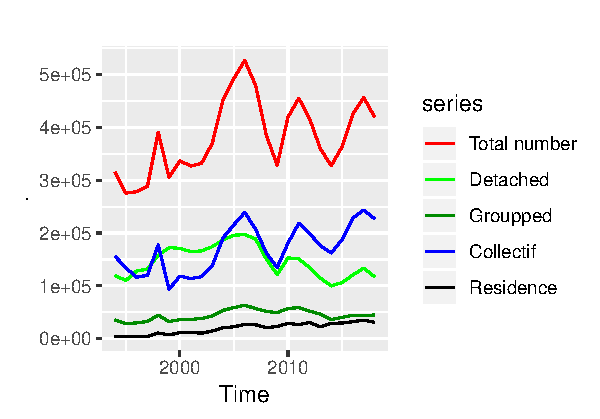
\includegraphics{presentation_files/figure-beamer/unnamed-chunk-16-1} 

}

\caption{Construction permits by housing type}\label{fig:unnamed-chunk-16}
\end{figure}

\normalsize

\FloatBarrier

\end{frame}

\begin{frame}{Transformed data for different housing types}
\protect\hypertarget{transformed-data-for-different-housing-types}{}

\FloatBarrier

\tiny

\begin{figure}[!htbp]

{\centering 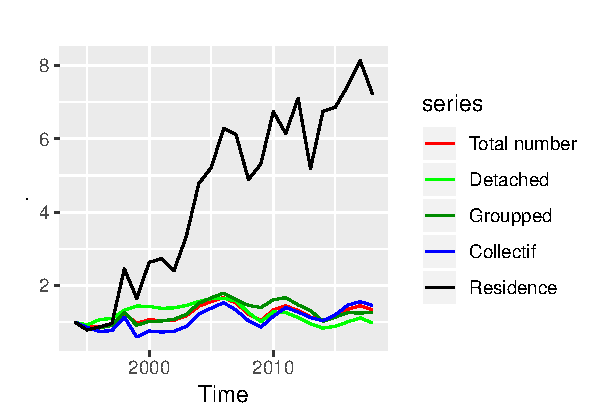
\includegraphics{presentation_files/figure-beamer/unnamed-chunk-17-1} 

}

\caption{Construction permits by housing type, index}\label{fig:unnamed-chunk-17}
\end{figure}

\normalsize

\FloatBarrier

\end{frame}

\hypertarget{data-analysis}{%
\section{Data analysis}\label{data-analysis}}

\begin{frame}{Analysis}
\protect\hypertarget{analysis}{}

We are going to procede in this section as follows :

\begin{itemize}
\tightlist
\item
  Cross-corelation study,
\item
  Autocorrelation study,
\item
  Partial autocorrelation study.
\end{itemize}

This analysis will be effectuated over the integrity of variables.

\end{frame}

\begin{frame}{Cross-correlation study}
\protect\hypertarget{cross-correlation-study}{}

In order to verify stationarity we use the following tests :

\begin{itemize}
\tightlist
\item
  augmented Dickey-Fuller test (ADF), which makes it possible to test
  the hypothesis of the non-stationarity of a time series;
\item
  Kwiatkowski-Phillips-Schmidt-Shin test (KPSS) to check stationarity on
  trend (KPSS-T) or level (KPSS-L).
\end{itemize}

These two tests allow us to verify the hypothesis of the stationarity of
the series studied and, if necessary, correct it by applying a
transformation on the series in question.

\end{frame}

\begin{frame}{Stationarity tests}
\protect\hypertarget{stationarity-tests}{}

\FloatBarrier

\tiny

\begin{table}[ht]
\centering
\begin{tabular}{rrrr}
  \hline
 & ADF & KPSS.T & KPSS.L \\ 
  \hline
GDP & 0.31 & 0.10 & 0.10 \\ 
  Interest rate & 0.17 & 0.10 & 0.10 \\ 
  Household spendings & 0.02 & 0.10 & 0.06 \\ 
  Household investments & 0.42 & 0.10 & 0.10 \\ 
  Number of permits & 0.01 & 0.10 & 0.10 \\ 
  Population $<$ 20 y.o. & 0.52 & 0.10 & 0.06 \\ 
  Population 20-59 y.o. & 0.67 & 0.10 & 0.01 \\ 
  Population $>$ 60 y.o. & 0.57 & 0.10 & 0.03 \\ 
   \hline
\end{tabular}
\caption{Stationarity tests, p-values} 
\end{table}

\normalsize

\FloatBarrier

\end{frame}

\begin{frame}{Differenced data}
\protect\hypertarget{differenced-data}{}

\FloatBarrier

\tiny

\begin{figure}[!htbp]

{\centering 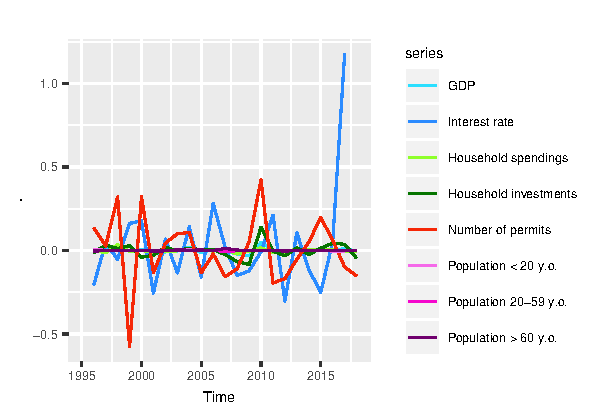
\includegraphics{presentation_files/figure-beamer/unnamed-chunk-21-1} 

}

\caption{Differenced time series}\label{fig:unnamed-chunk-21}
\end{figure}

\normalsize

\FloatBarrier

\end{frame}

\begin{frame}{Stationarity reverification}
\protect\hypertarget{stationarity-reverification}{}

\FloatBarrier

\tiny

\begin{table}[ht]
\centering
\begin{tabular}{rrrr}
  \hline
 & ADF & KPSS.T & KPSS.L \\ 
  \hline
GDP & 0.03 & 0.10 & 0.10 \\ 
  Interest rate & 0.29 & 0.10 & 0.10 \\ 
  Household spendings & 0.04 & 0.10 & 0.10 \\ 
  Household investments & 0.06 & 0.10 & 0.10 \\ 
  Number of permits & 0.01 & 0.10 & 0.10 \\ 
  Population $<$ 20 y.o. & 0.27 & 0.10 & 0.10 \\ 
  Population 20-59 y.o. & 0.57 & 0.10 & 0.10 \\ 
  Population $>$ 60 y.o. & 0.55 & 0.08 & 0.10 \\ 
   \hline
\end{tabular}
\caption{Stationarity tests, p-values} 
\end{table}

\normalsize

\FloatBarrier

\end{frame}

\begin{frame}{Cross-correlation study}
\protect\hypertarget{cross-correlation-study-1}{}

\FloatBarrier

\tiny

\begin{figure}[!htbp]

{\centering 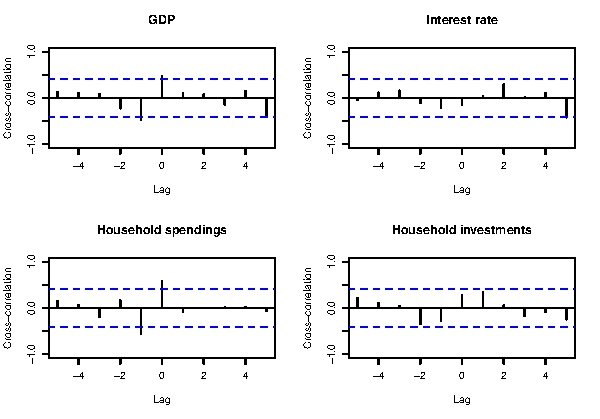
\includegraphics{presentation_files/figure-beamer/unnamed-chunk-24-1} 

}

\caption{Cross-correlation}\label{fig:unnamed-chunk-24}
\end{figure}

\normalsize

\FloatBarrier

\end{frame}

\begin{frame}{Autocorrelation}
\protect\hypertarget{autocorrelation}{}

\FloatBarrier

\tiny

\begin{figure}[!htbp]

{\centering 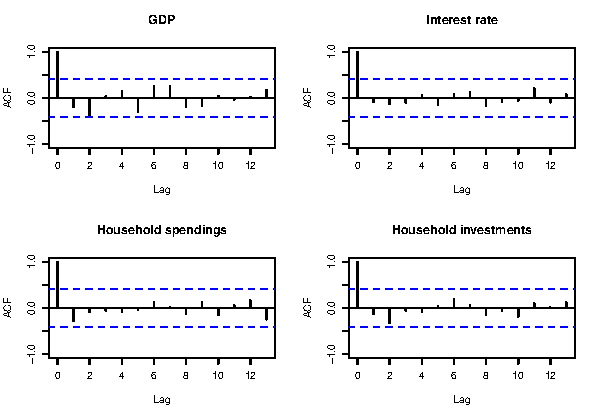
\includegraphics{presentation_files/figure-beamer/unnamed-chunk-25-1} 

}

\caption{Autocorrelation}\label{fig:unnamed-chunk-25}
\end{figure}

\normalsize

\end{frame}

\begin{frame}{Partial autocorrelation}
\protect\hypertarget{partial-autocorrelation}{}

\FloatBarrier

\tiny

\begin{figure}[!htbp]

{\centering 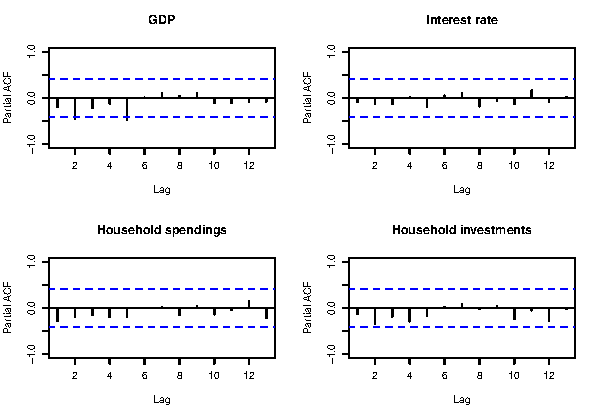
\includegraphics{presentation_files/figure-beamer/unnamed-chunk-26-1} 

}

\caption{Partial autocorrelation}\label{fig:unnamed-chunk-26}
\end{figure}

\normalsize

\FloatBarrier

\end{frame}

\hypertarget{modelisation}{%
\section{Modelisation}\label{modelisation}}

\begin{frame}{Different models}
\protect\hypertarget{different-models}{}

\begin{itemize}
\tightlist
\item
  Simple linear models (OLS),
\item
  Time series models (ARIMA),
\item
  Adcanced time series vector models (VAR),
\item
  Alternative linear models, accounting for causality effects.
\end{itemize}

\end{frame}

\begin{frame}{Model comparison}
\protect\hypertarget{model-comparison}{}

\tiny
\begin{table}[H]
\begin{tabular}{p{2cm} | p{4cm} | p{4cm}}
\hline \\[-1.8ex]
Model & 
    Advantages & 
        Disadvantages \\
\hline
OLS & 
    Simple to implement & 
        Unable to predict future values without acces to exogenous variables values in future \\
\hline
ARIMA & 
    Relatively simple  
    Allows to predict future values for several periods &
        \makecell{Does not take into account supplimentary information \\
        Requires stationary time series data} \\
\hline
VAR & 
    Even longer prediction horizon & 
        \makecell{Multiple restriction on data structure : \\
        - Stationarity, \\
        - No cointegration.} \\
\hline
OLS and causality & 
    \makecell{Gives predictions for short intervals (1 or 2 periods) \\
    No limiting restrictions on the data used} &
        Only short-term predictions are possible \\
\hline
\end{tabular}
\normalsize
\caption{Different models' specification}
\end{table}

\end{frame}

\hypertarget{linear-models}{%
\section{Linear models}\label{linear-models}}

\begin{frame}{OLS estimations}
\protect\hypertarget{ols-estimations}{}

In this part we explore direct links between varibales without wausality
imlications.

\FloatBarrier

\tiny

\begin{table}[!htbp]
\begin{center}
\begin{tabular}{l c c c c c }
\hline
 & Model 1 & Model 2 & Model 3 & Model 4 & Model 5 \\
\hline
GDP                   & $4.38^{*}$ & $5.40^{*}$ & $1.10$   & $2.00$   & $2.98$   \\
                      & $(2.10)$   & $(2.22)$   & $(4.89)$ & $(4.94)$ & $(4.93)$ \\
Interest rate         &            & $-0.17$    &          & $-0.18$  & $-0.18$  \\
                      &            & $(0.13)$   &          & $(0.14)$ & $(0.14)$ \\
Household spendings   &            &            & $3.13$   & $1.77$   & $3.38$   \\
                      &            &            & $(3.86)$ & $(4.02)$ & $(4.17)$ \\
Household investments &            &            & $0.56$   & $0.92$   & $0.68$   \\
                      &            &            & $(1.47)$ & $(1.49)$ & $(1.48)$ \\
Time                  &            &            &          &          & $0.01$   \\
                      &            &            &          &          & $(0.01)$ \\
\hline
R$^2$                 & 0.17       & 0.24       & 0.20     & 0.26     & 0.32     \\
Adj. R$^2$            & 0.13       & 0.16       & 0.08     & 0.10     & 0.12     \\
Num. obs.             & 24         & 23         & 24       & 23       & 23       \\
RMSE                  & 0.14       & 0.14       & 0.14     & 0.14     & 0.14     \\
\hline
\multicolumn{6}{l}{\scriptsize{$^{***}p<0.001$, $^{**}p<0.01$, $^*p<0.05$}}
\end{tabular}
\caption{OLS models comparison}
\label{table:coefficients}
\end{center}
\end{table}

\normalsize

\FloatBarrier

\end{frame}

\hypertarget{time-series}{%
\section{Time series}\label{time-series}}

\begin{frame}{Time series presentation}
\protect\hypertarget{time-series-presentation}{}

\FloatBarrier

\tiny

\begin{figure}[!htbp]

{\centering 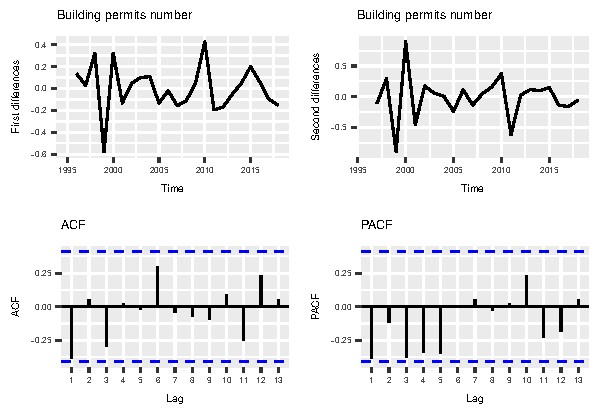
\includegraphics{presentation_files/figure-beamer/unnamed-chunk-33-1} 

}

\caption{Descriptive graphics}\label{fig:unnamed-chunk-33}
\end{figure}

\normalsize

\FloatBarrier

\end{frame}

\begin{frame}{ARMA modelisation}
\protect\hypertarget{arma-modelisation}{}

\FloatBarrier

\tiny

\begin{table}[!htbp]
\begin{center}
\begin{tabular}{l c c c c c }
\hline
 & ARMA(1,0) & ARMA(0,1) & ARMA(1,1) & ARMA(1,2) & ARMA(2,2) \\
\hline
AR(1)          & $-0.38$  &          & $0.04$   & $-0.96$  & $-0.81$  \\
               & $(0.19)$ &          & $(0.22)$ & $(0.15)$ & $(0.28)$ \\
AR(2)          & $0.00$   & $-0.00$  & $-0.00$  & $-0.00$  & $-0.00$  \\
               & $(0.03)$ & $(0.00)$ & $(0.00)$ & $(0.00)$ & $(0.00)$ \\
Intercept      &          & $-1.00$  & $-1.00$  & $-0.09$  & $-0.12$  \\
               &          & $(0.12)$ & $(0.12)$ & $(0.24)$ & $(0.23)$ \\
MA(1)          &          &          &          & $-0.91$  & $-0.88$  \\
               &          &          &          & $(0.24)$ & $(0.22)$ \\
MA(2)          &          &          &          &          & $0.13$   \\
               &          &          &          &          & $(0.22)$ \\
\hline
AIC            & -4.98    & -13.34   & -11.38   & -9.76    & -8.11    \\
Log Likelihood & 5.49     & 9.67     & 9.69     & 9.88     & 10.06    \\
\hline
\multicolumn{6}{l}{\scriptsize{$^{***}p<0.001$, $^{**}p<0.01$, $^*p<0.05$}}
\end{tabular}
\caption{Comparaison des modèles ARMA}
\label{table:coefficients}
\end{center}
\end{table}

\normalsize

\FloatBarrier

\end{frame}

\hypertarget{vector-models}{%
\section{Vector models}\label{vector-models}}

\begin{frame}{VAR modelisation}
\protect\hypertarget{var-modelisation}{}

\FloatBarrier

\tiny

\normalsize

\FloatBarrier

\end{frame}

\hypertarget{alternatives}{%
\section{Alternatives}\label{alternatives}}

\begin{frame}{Review of cross-correlations, part 1}
\protect\hypertarget{review-of-cross-correlations-part-1}{}

\FloatBarrier

\tiny

\begin{figure}[!htbp]

{\centering 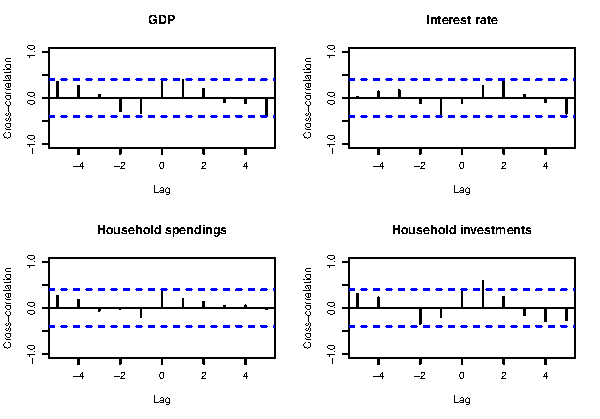
\includegraphics{presentation_files/figure-beamer/unnamed-chunk-39-1} 

}

\caption{Cross-correlation}\label{fig:unnamed-chunk-39}
\end{figure}

\normalsize

\FloatBarrier

\end{frame}

\begin{frame}{Review of cross-correlations, part 2}
\protect\hypertarget{review-of-cross-correlations-part-2}{}

\FloatBarrier

\tiny

\begin{figure}[!htbp]

{\centering 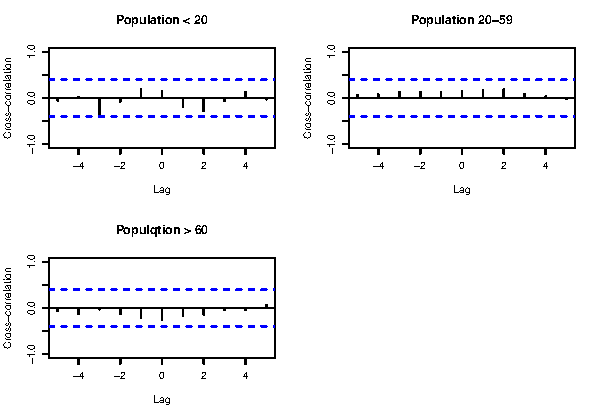
\includegraphics{presentation_files/figure-beamer/unnamed-chunk-40-1} 

}

\caption{Cross-correlation}\label{fig:unnamed-chunk-40}
\end{figure}

\normalsize

\FloatBarrier

\end{frame}

\hypertarget{conclusion}{%
\section{Conclusion}\label{conclusion}}

\begin{frame}{Proceedings}
\protect\hypertarget{proceedings}{}

\begin{itemize}
\tightlist
\item
  Separate study of different permits types,
\item
  Alternative linear regression implementation (that is similar to
  ARDL),
\item
  Study of trimestrial data,
\item
  Rapport finalisation,
\item
  Delivrables preparation :

  \begin{itemize}
  \tightlist
  \item
    Excel automated model,
  \item
    Final rapport,
  \item
    R code organisation,
  \item
    Database documentation.
  \end{itemize}
\end{itemize}

\end{frame}

\end{document}
